\documentclass[11pt, oneside]{article}   	% use "amsart" instead of "article" for AMSLaTeX format
\usepackage{geometry}                		% See geometry.pdf to learn the layout options. There are lots.
\geometry{letterpaper}                   		% ... or a4paper or a5paper or ... 
%\geometry{landscape}                		% Activate for for rotated page geometry
%\usepackage[parfill]{parskip}    		% Activate to begin paragraphs with an empty line rather than an indent
\usepackage{graphicx}				% Use pdf, png, jpg, or eps� with pdflatex; use eps in DVI mode
								% TeX will automatically convert eps --> pdf in pdflatex		
\usepackage{amssymb}
\usepackage{amsmath}
\usepackage{parskip}
\usepackage{color}
\usepackage{hyperref}

\title{Fourier series, introduction}
%\author{The Author}
%\section{}
%\subsection*{}
\date{}							% Activate to display a given date or no date

\graphicspath{{/Users/telliott_admin/Dropbox/Tex/png/}}
% \begin{center} 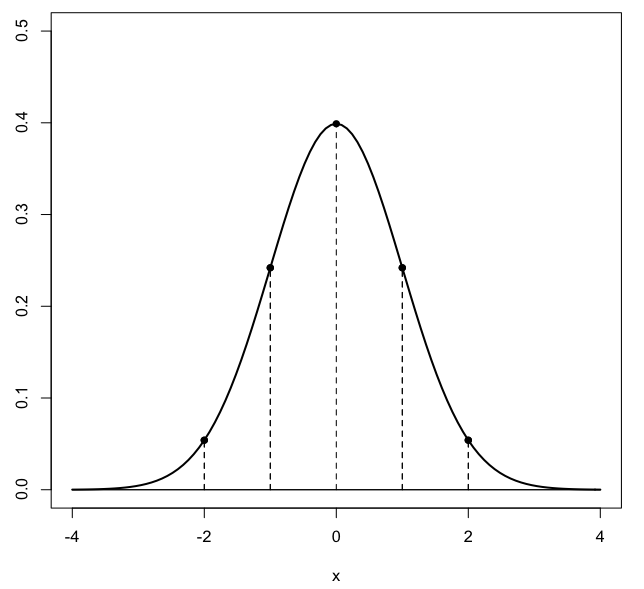
\includegraphics [scale=0.4] {gauss3.png} \end{center}
\begin{document}
\maketitle
\Large
If we consider the two series $\cos kx$ and $\sin kx$:
\[ \cos x, \cos 2x, \cos 3x \dots \cos kx \]
\[ \sin x, \sin 2x, \sin 3x \dots \sin kx \]
where $k \in \mathbb{N} \ \ (k = 1,2,3 \dots)$

\emph{Any} function in this set is \emph{orthogonal} to each of the others, by which we mean that:  
\[ \int f(x) \ g(x) \ dx = 0 \]
Thus, considering the cosine-cosine pair, for $m,n \in \mathbb{N}$:
\[ \int \cos mx \cos nx \ dx =
\begin{cases}
0, & m \ne n \\
\pi, & m = n \ne 0 \\
2 \pi, & m = n = 0
\end{cases}
\]
The usual intervals over which we will integrate are $[0,2\pi]$ and especially $[-\pi,\pi] \ $--- these are bounds that are each a multiple of $\pi$ and the length of the interval is equal to $2 \pi$.

The sine-sine pair is almost the same, except that the only non-zero case is $m = n \ne 0$, where the result is $\pi$.
\[ \int \sin mx \sin nx \ dx =
\begin{cases}
0, & m \ne n \\
\pi, & m = n \ne 0 \\
0, & m = n = 0
\end{cases}
\]

And finally, for the sine-cosine pair all cases are zero.  

If you want to be really fancy, you can use what's called the Kronecker Delta:
\[
\delta_{ij} = 
\begin{cases}
0 & \text{for} \ i \ne j \\
1 & \text{for} \ i = j
\end{cases}
\]
Then
\[ \int \cos mx \cos nx \ dx = \pi \delta_{mn}  \]
\[ \int \sin mx \sin nx \ dx = \pi \delta_{mn} \]
\[ \int \cos mx \sin nx \ dx = 0 \]

\url{http://mathworld.wolfram.com/FourierSeries.html}

(Although this doesn't cover the special behavior of the first function for $m=n=0$).

We will use these facts to develop Fourier series that approximate $f(x)$ as an infinite sum of sine and cosine functions.

\subsection*{cosine-cosine}
Before we do that, let's look at all three integrals in more detail.

Recalling the cosine addition formulas:
\[ \cos (s + t) = \cos s \cos t - \sin s \sin t \]
\[ \cos (s - t )= \cos s \cos t + \sin s \sin t \]
Add them together and multiply through by $1/2$:
\[ \frac{1}{2} \ [ \ \cos (s + t) + \cos (s - t)  \ ] \ = \cos s \cos t  \]
So then
\[ \int \cos mx \cos nx \ dx \]
\[ = \frac{1}{2}  \int  \cos (m+n) x + \cos (m-n)x \ dx \]

For the first case, $m=n=0$, we have
\[ \frac{1}{2} \int \cos 0 + \cos 0 \ dx = \int dx \]
and so we obtain just $x$ evaluated between some limits.

We will choose as the bounds $[-\pi,\pi]$. 
\[ \int_{-\pi}^{\pi}  dx = 2 \pi \]

For this integral ($\int dx$) no matter what limits separated by $2 \pi$ we might choose, whether $\int_0^{2\pi}$ or any $\int_{-\pi}^{\pi}$ or $\int_a^{a+2\pi}$, we would obtain $2\pi$ for the result.

On the other hand, if $m=n \ne 0$, then in exactly the same way, we obtain the value of $\pi$ as the result from the second term (remember the factor of $\frac{1}{2}$).  The first term is zero, as follows:

For any non-zero integer $k$, whether $k = m + n$ or $k = m - n$ (as we will have below):

\[ \int_{-\pi}^{\pi} \cos k x \ dx =  \frac{\sin k x}{k} \ \bigg |_{-\pi}^{\pi} \]

whether we choose bounds $\int_0^{2\pi}$ or $\int_{-\pi}^{\pi}$ or some other $[a, a + 2 \pi]$, we obtain $0$ for the result.

Graph the sine function between any bounds separated by $2 \pi$ and the area of the function above zero is equal to the area below zero, no matter what the value of $a$.  This is also true for the cosine.

\subsection*{sine-sine}
\[ \int \sin mx \sin nx \ dx \]
Go back to the sum of cosines above and subtract the first equation from the second to obtain
\[ \frac{1}{2} (\cos s - t - \cos s + t) = \sin s \sin t \]
Hence
\[ \int \sin mx \sin nx \ dx \]
\[ = \frac{1}{2}  \int  \cos (m-n) x - \cos (m+n)x \ dx \]
This is very similar to what we had before.  The difference is the minus sign.  Here, if $m=n=0$ the two terms are identical ($\cos (0) = 1$) and they cancel.  

On the other hand, if $m=n\ne 0$ we get a value of $\pi$ from the first term as before.  

For any non-zero $k$ in the argument to the cosine, we have
\[ \int_{-\pi}^{\pi} \cos kx \ dx = \frac{\sin kx}{k} \ \bigg |_{-\pi}^{\pi} \]
which, again as we saw before is zero for any $\int_a^{a+2 \pi}$.

\subsection*{sine-cosine}
One way to do this is to remember the addition formula for sine:
\[ \sin (s + t) = \sin s \cos t + \sin t \cos s \]
\[ \sin (s - t) = \sin s \cos t - \sin t \cos s \]
\[ \frac{1}{2} \ [ \ \sin(s+t) + \sin(s-t) \ ] \ = \sin s \cos t  \]
So we have
\[ \int \sin mx \cos nx \ dx \]
\[ =  \frac{1}{2} \int \sin(m+n)x + \sin(m-n)x \ dx \]

Here, the case with $m=n=0$ is $\int \sin(0) \ dx$ which is just $0$.

For $m=n \ne 0$, the second term is zero and the first is
\[ \int_a^b \sin kx \ dx = - \frac{\cos kx}{k} \ \bigg |_{-\pi}^{\pi} \]
which is zero for any $\int_a^{a+2 \pi}$.

Lastly, for $m \ne n$ we obtain
\[ \int_{-\pi}^{\pi}\sin(m+n)x + \sin(m-n)x \ dx \]
\[ = - \frac{\cos (m+n)x}{m+n} - \frac{\cos (m-n)x}{m-n} \ \bigg |_{-\pi}^{\pi} \]
which is zero for any $\int_a^{a+2 \pi}$ for the same reason.  Hence all the cases for sine-cosine are zero.

\subsection*{writing a series}

Now, suppose we try to represent a function $f(x)$ as a series using sine and cosine
\[ f(x) = \frac{a_0}{2} + a_1 \cos x + a_2 \cos 2x + \dots + b_1 \sin x + b_2 \sin 2x + \dots \]
We need to determine the cofactors (and we'll see the reason for the factor of $1/2$ on $a_0$ shortly).  If we multiply both sides by $\cos mx$ and integrate over the interval $[-\pi,\pi]$, all of the infinite number of terms on the right-hand side vanish except for the one with cofactor $a_m$:

\[ \int_{-\pi}^{\pi} f(x) \ \cos mx \ dx   =  a_m \int_{-\pi}^{\pi} \cos mx \cos mx \ dx \]

Remember from the previous section that for $m=n \ne 0$ the right-hand integral is equal to $\pi$ so
\[ \int_{-\pi}^{\pi} f(x) \ \cos mx \ dx   =   \pi a_m \]
Thus
\[ a_m = \frac{1}{\pi} \int_{-\pi}^{\pi} f(x) \ \cos mx \ dx \]
Similarly, we can determine the coefficients $b_m$ by multiplying by $\sin mx$ and integrating.  By the same reasoning as before, we obtain:
\[ b_m = \frac{1}{\pi}\int_{-\pi}^{\pi} f(x) \ \sin mx \ dx \]
Last, we have $m = 0$, 
\[ \int_{-\pi}^{\pi} f(x) \cos 0 \ dx = \frac{1}{2} \ \int_{-\pi}^{\pi} a_0 \cos 0 \ dx \]
\[ \int_{-\pi}^{\pi} f(x) \ dx = \frac{a_0}{2} \ 2 \pi = a_0 \pi \]
\[ a_0 = \frac{1}{\pi} \ \int_{-\pi}^{\pi} f(x) \ dx \]
We can use any interval of length $2 \pi$, here it was $[-\pi,\pi]$ as given here.

For reference then, the cofactors are
\[ \begin{cases}
a_0 =  \frac{1}{\pi}  \int_{-\pi}^{\pi} f(x) \ dx \\
a_m = \frac{1}{\pi}  \int_{-\pi}^{\pi} \cos mx f(x) \ dx \\
b_m = \frac{1}{\pi}  \int_{-\pi}^{\pi} \sin mx f(x) \ dx \\
\end{cases}
\]

\subsection*{application: odd step function}
Consider the step function:
\[ \begin{cases}
f(x) = -1 & x < 0 \\
f(x) = 1 &  x > 0
\end{cases}
\]
This function is an \emph{odd} function:  $f(x) = -f(-x)$, while the cosine is an even function ($\cos x = \cos -x$).  An even function times an odd function is an odd function.  The integral of an odd function that is symmetric across zero vanishes.

Therefore, on the interval $[-\pi,\pi]$, all the terms with cosine vanish:
\[  a_m = \frac{1}{\pi} \int_{-\pi}^{\pi} f(x) \ \cos mx \ dx = 0  \]
To drive this point home:
\[ = \frac{1}{\pi} \ [ \ \int_{-\pi}^{0} f(x) \ \cos mx \ dx + \int_{0}^{\pi} f(x) \ \cos mx \ dx \ ] \]
For every value $x$ from $0 < x  < \pi$ from the second term and its $f(x)$, there is a value $f(-x)$ from the first term with opposite sign, multiplied by the same value $\cos( -mx) = \cos mx$, and they all cancel.

Thus the coefficients that do remain are those for sine:
\[ b_m = \frac{1}{\pi} \ [ \ \int_{-\pi}^{0} f(x) \ \sin mx \ dx + \int_{0}^{\pi} f(x) \ \sin mx \ dx \ ] \]
\[ = \frac{1}{\pi}  \ [ \ - \int_{-\pi}^{0} \ \sin mx \ dx + \int_{0}^{\pi} \ \sin mx \ dx \ ] \]
For the sine function, the integral over $[-\pi,0]$ is equal and opposite in sign to the integral over $[0,\pi]$
\[ = \frac{1}{\pi}  \ [ \ \int_{0}^{\pi} \ \sin mx \ dx + \int_{0}^{\pi} \ \sin mx \ dx \ ] \]
\[ \frac{2}{\pi}  \int_{0}^{\pi} \ \sin mx \ dx \] 
\[ = -\frac{2}{m\pi} \ [ \ \cos mx \ \bigg  |_{0}^{\pi} \ ] \]
For even $m$, the terms ($\cos 2\pi, \cos 4 \pi \dots$) are all the same as at the lower bound, leaving us with zero, while for odd $m$ we get a factor of $-2$ from the integral so the whole thing is
\[ b_m = \frac{4}{m \pi} \]
We also have
\[ a_0 =  \frac{1}{\pi}  \int_{-\pi}^{\pi} f(x) \ dx \]
\[ = \frac{1}{\pi}  \ [ \  \int_{-\pi}^{0} f(x) \ dx +  \int_{0}^{\pi} f(x) \ dx \ ]  \]
\[ = \frac{1}{\pi}  ( - \pi + \pi ) = 0 \]
If that was confusing, just remember that $f(x)$ is odd, and the interval of integration is symmetric around $0$.

So the series is $4/\pi$ times the values $\sin kx/k$ for odd $k$:
\[ f(x) = \frac{4}{\pi} \ [ \ \sin x + \frac{1}{3} \sin 3x + \frac{1}{5} \sin 5x + \frac{1}{7} \sin 7x + \dots \ ]  \]
which we can approximate with four terms
\begin{center}
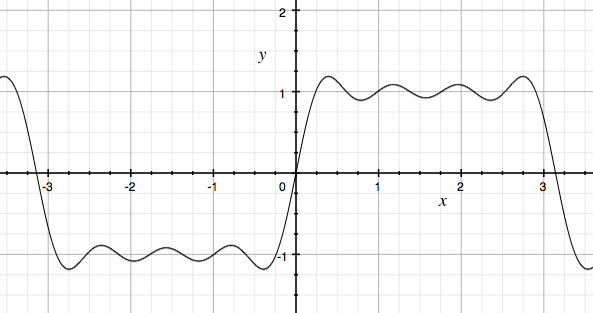
\includegraphics [scale=0.5] {fourier1.png}
\end{center}
Notice there is one little hump in the step for each term we include.

\subsection*{application: even step function}
Consider the step function centered on zero:
\[ \begin{cases}
f(x) = 1 & -\frac{\pi}{2} < x < \frac{\pi}{2}  \\
f(x) = 0 & \text{otherwise}
\end{cases}
\]
Since this is an even function, all the $b_m$ will be zero:
\[ b_m = \frac{1}{\pi}  \int_{-\pi}^{\pi} f(x) \ \sin mx \ dx = 0 \]
The cosine terms are:
\[ a_m = \frac{1}{\pi}  \int_{-\pi}^{\pi} f(x) \ \cos mx \ dx = 0 \]
$f(x) = 0$ outside $[-\pi/2,\pi/2]$:
\[ = \frac{1}{\pi}  \int_{-\pi/2}^{\pi/2} f(x) \ \cos mx \ dx \]
$f(x) = 1$ inside $[-\pi/2,\pi/2]$:
\[ = \frac{1}{\pi}  \int_{-\pi/2}^{\pi/2} \ \cos mx \ dx \]
Cosine is an even function so:
\[ = \frac{2}{\pi}  \int_{0}^{\pi/2} \cos mx \ dx \]
\[ = \frac{2}{\pi m} \sin mx \ \bigg |_{0}^{\pi/2}   \]
Only the odd terms survive, and these terms alternate in sign.  Check $a_0$
\[ a_0 = \frac{1}{2 \pi}  \int_{-\pi}^{\pi} f(x) \ dx \]
\[ = \frac{1}{\pi}  \int_{-\pi/2}^{\pi/2} \ dx  \]
\[ = 1 \]
Recall that the $a_0$ term has a coefficient of $\frac{1}{2}$
\[ f(x) = \frac{1}{2} + \frac{2}{\pi} \ [ \ \cos x - \frac{\cos 3x}{3} + \frac{\cos 5x}{5} + \dots \ ] \]

\begin{center}
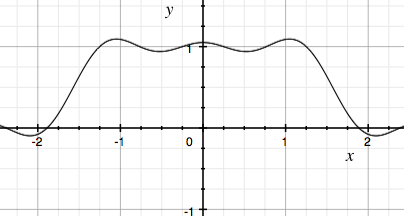
\includegraphics [scale=0.5] {fourier2.png}
\end{center}

\subsection*{application:  f(x) = x}
This function is an odd function:  $f(x) = -f(-x)$, while the cosine is an even function ($\cos x = \cos -x$).  An even function times an odd function is an odd function, and so all the cosine terms vanish (between $[-\pi,\pi]$, as before.

Thus the coefficients that do remain are those for sine:
\[ b_m = \frac{1}{\pi} \ [ \ \int_{-\pi}^{\pi} f(x) \ \sin mx \ dx \ ] \]
\[ = \frac{1}{\pi} \ [ \ \int_{-\pi}^{\pi} x \ \sin mx \ dx \ ] \]

We can integrate $x \sin x$ using integration by parts, or we can just guess:
\[ \int x \sin x \ dx = - x \cos x + \sin x \]
Check
\[ \frac{d}{dx} \ - x \cos x + \sin x = x \sin x - \cos x + \cos x = x \sin x \]
We do have that factor of $m$
\[ \frac{d}{dx} \ \frac{1}{m} ( - x \cos mx +  \sin mx) \] 
\[ = x \sin mx - \frac{\cos mx}{m} + \frac{\cos mx}{m} = x \sin mx \]

The limits are $[-\pi,\pi]$.  We do not forget the factor of $1/\pi$ in front.
\[ b_m = \frac{1}{\pi m} ( - x \cos mx +  \sin mx) \ \bigg |_{-\pi}^{\pi} \]

Now the second term $\sin k \pi$ is zero for any integer $k$.  That leaves
\[ b_m = \frac{1}{\pi m} ( - x \cos mx )\ \bigg |_{-\pi}^{\pi} \]
\[ = -\frac{1}{\pi m} ( x \cos mx )\ \bigg |_{-\pi}^{\pi} \]
\[ = -\frac{1}{\pi m} \ [ \ \pi \cos m \pi - (-\pi) \cos m (- \pi )\ ] \ \]
\[ = -\frac{1}{\pi m} \ [ \ \pi \cos m \pi + \pi \cos m (- \pi )\ ] \ \]
\[ = -\frac{1}{\pi m} \ [ \ \pi \cos m \pi + \pi \cos m \pi \ ] \ \]
\[ = \frac{-2}{\pi m} \ [ \ \pi \cos m \pi \ ] \ \]

\[ = -\frac{2}{m}  \cos m\pi \ \]

The terms for odd $m$ are
\[ a_m = \frac{2}{m} \]
while the even terms are
\[ a_m = - \frac{2}{m} \]

For $a_0$:
\[ a_0 = \frac{1}{\pi} \int_{-\pi}^{\pi} x \ dx \]
$x$ is an odd function so the integral is zero
\[ = \frac{1}{2 \pi} x^2 \ \bigg |_{-\pi}^{\pi} = 0 \]
So finally we have that 
\[ f(x) = 2 \ [ \ \sin x - \frac{\sin 2x}{2} + \frac{\sin 3x}{3} - \frac{\sin 4x}{4} + \dots \ ] \]
Here are 10 terms
\begin{center}
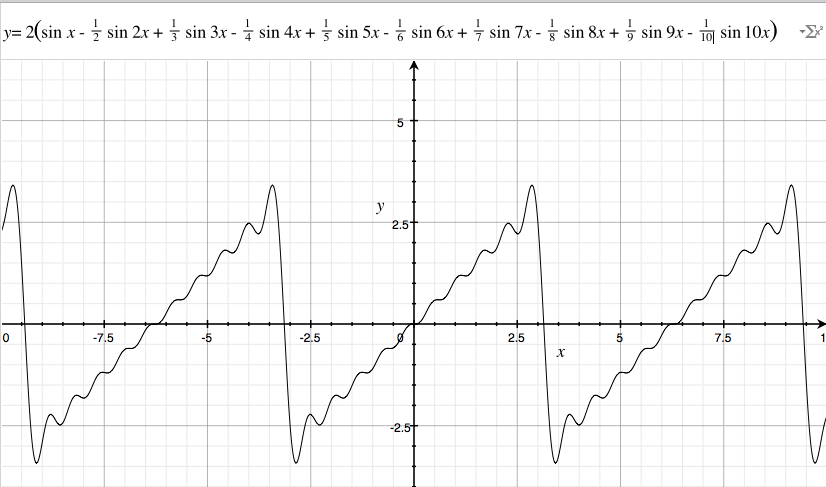
\includegraphics [scale=0.5] {fourier3.png}
\end{center}

\subsection*{complex exponential}

The derivation that we did previously can be accomplished in a simpler way using the complex exponential (Euler's formula):
\[ e^{i\theta} = \cos \theta + i \sin \theta \]
switching to $x$
\[ e^{ix} = \cos x + i \sin x \]
\[ e^{-ix} = \cos x - i \sin x \]
Adding or subtracting gives:
\[ \cos x = \frac{1}{2} (e^{ix} + e^{-ix}) \]
\[ \sin x = \frac{1}{2i} (e^{ix} - e^{-ix}) \]

So why don't we investigate the orthogonality of the function $e^{ikx}$ where $k, m \in \mathbb{N}$:
\[ \int_{-\pi}^{\pi} e^{ikx} e^{-imx} \ dx \]
What we find is that, as before, the result is zero when $k \ne m$:
\[ \int_{-\pi}^{\pi} e^{ikx} e^{-imx} \ dx  =  \int_{-\pi}^{\pi} e^{i(k-m)x} \ dx \]
\[ = \frac{ e^{i(k-m)x}}{k-m} \ \bigg |_{-\pi}^{\pi} \]
Convert back to $\sin$ and $\cos$ to see the result more easily:
\[ \int_{-\pi}^{\pi}  e^{i(k-m)x } = \frac{1}{i(k-m)} \ [ \ \cos (k-m)x + i \sin (k-m)x \ ] \ \bigg |_{-\pi}^{\pi} \]

Consider $n = k-m$.  Since $n$ is an integer, the sine term is zero ($\sin n\pi = 0$).  If $n$ is odd, the cosine term is equal to $1$ at both the upper and lower bounds, while if $n$ is even the cosine term is equal to $-1$ at both the upper and lower bounds, so the difference is zero in both cases.

Actually, the total integral is zero for any bounds $\int_a^{a+2\pi}$ since
\[ \cos a = \cos (a + 2 \pi), \ \ \  \sin a = \sin (a + 2 \pi) \]

On the other hand, if $k=m$ then
\[ \int_0^{2\pi} e^{ikx} e^{-imx} \ dx = \int_0^{2\pi} \ dx = 2 \pi \]
So again, we will try to approximate $f(x)$ by a series with terms $c_k e^{ikx}$
\[ f(x) =  \sum_{k=-\infty}^{\infty} c_k e^{ikx}  \]
Notice that in this series we have negative integer $k$ as well.

To determine the coefficient $c_k$, multiply both sides by $e^{-ikx}$ and integrate over the interval $[-\pi,\pi]$.  As before, all the terms of the series except those with $c_k e^{ikx} e^{-ikx}$ drop out and the result for the one remaining is just $c_k$ times $2 \pi$ so:
\[ c_k = \frac{1}{2 \pi} \int_{-\pi}^{\pi} f(x) e^{-ikx} \ dx \]
\[ c_0 =  \frac{1}{2 \pi} \int_{-\pi}^{\pi} f(x) \ dx \]

\subsection*{application: odd step function}
Consider the step function:
\[ \begin{cases}
f(x) = -1 & x < 0 \\
f(x) = 1 &  x > 0
\end{cases}
\]

For $k \in \{ \dots -3,-2,-1,0,1,2,3 \dots \}$:
\[ c_k = \frac{1}{2\pi} \int_{-\pi}^{\pi} f(x) \ e^{-ikx} \ dx \]
Hamming solves this quickly but I couldn't follow a key step.

Let us go more slowly and carefully and write it as the cosine plus sine:
\[ c_k = \frac{1}{2\pi} \int_{-\pi}^{\pi} f(x) \ [ \ \cos -kx + i \sin -kx \ ] \ dx \]
\[ c_k = \frac{1}{2\pi} \int_{-\pi}^{\pi} f(x) \ [ \ \cos kx - i \sin kx \ ] \ dx \]

$f(x)$ is an odd function, while cosine is an even function, hence the cosine term vanishes when integrated from $\int_{-\pi}^{\pi}$, so we have
\[ c_k = - \frac{i}{2\pi} \int_{-\pi}^{\pi} f(x) \sin kx \ dx \]
Substitute for $f(x)$
\[ = -\frac{i}{2\pi} \ [ \ \int_{-\pi}^{0} - \sin kx \ dx + \int_{0}^{\pi} \sin kx \ dx \ ]  \]
\[ = - \frac{i}{2\pi k} \ [ \ \cos kx \ \bigg |_{-\pi}^{0} \ -  \cos kx \ \bigg |_{0}^{\pi} \ ]  \]

Consider the two evaluations separately:
\[ \cos kx \ \bigg |_{-\pi}^{0} \]
\[ \cos 0 - \cos (-k\pi) = 1 - \cos k \pi \]
For even $k$ this is $1-1 = 0$.  Alternatively just recall that the integral for sine or cosine over any interval of length $2 \pi$ is equal to $0$.  So all the even $k$ terms drop out.

For odd $k$ this is $1-  (-1) = 2$.

Similarly
\[ -  \cos kx \ \bigg |_{0}^{\pi} \]
for even $k$ this is $-(1 - 1) = 0$, and again there are no even terms.  For odd $k$ we have $-(-1 - 1) = 2$.  Adding them together, the total is $4$ and we have then:
\[ c_k = -\frac{2i}{\pi k}  \]

so our series for $f(x)$ is
\[ f(x) = \sum c_k e^{ikx} \]
\[ = -\frac{2i}{\pi k} \ (\cos kx + i \sin kx ) \]

At this point, we recall that the sum is over both negative and positive $k$.  So if we consider the terms with the same absolute value $|k|$ as a pair, replace $k$ with $|k|$ and put in minus signs appropriately.

For the first term in each pair we have $-k$, which gives $\cos -kx = \cos kx$ and $\sin -kx = - \sin kx$ so we obtain:
\[ = -\frac{2i}{\pi(- k)}  ( \cos kx - i \sin kx ) - \frac{2i}{\pi k} (\cos kx + i\sin kx ) \]
\[ = \frac{2i}{\pi k}  ( \cos kx - i \sin kx ) - \frac{2i}{\pi k} (\cos kx + i\sin kx ) \]
We see that the imaginary (cosine) terms cancel.  The result is purely real has the form
\[ = \frac{2}{\pi k} \sin kx + \frac{2}{\pi k} \sin kx \]
\[ = \frac{4}{\pi k}  \sin kx \]
for odd $k$ only.  That gives
\[ f(x) =  \sum \frac{4}{\pi}  \ \cdot \frac{\sin kx}{k} \]
\[ =  \frac{4}{\pi} \ [ \  \frac{\sin x}{1} +  \frac{\sin 3x}{3}  +  \frac{\sin 5x}{5} + \dots \]

Compare with what we had before:
\[ f(x) = \frac{4}{\pi} \ [ \ \sin x + \frac{1}{3} \sin 3x + \frac{1}{5} \sin 5x + \frac{1}{7} \sin 7x + \dots \ ]  \]

Now the only issue is that we have ignored $c_0$ so far.

Recall
\[ c_0 =  \frac{1}{2 \pi} \int_{-\pi}^{\pi} f(x) \ dx \]
Since $f(x)$ switches value from $-1$ to $+1$ at $0$, we split the integral and substitute for $f(x)$
\[ = - \frac{1}{2 \pi} \int_{-\pi}^{0} \ dx +  \frac{1}{2 \pi} \int_{0}^{\pi} \ dx  \]
The second term is clearly $1/2$, while the first integral is
\[ x \ \bigg |_{-\pi}^{0} = 0 - (- \pi) = \pi \]
times $-1/2 \pi$, which equals $-1/2$ and cancels the second term.  So we have that $c_0 = 0$.

This is a \emph{lot} harder than Hamming's sketch of the proof, but he had a step I couldn't justify.  We reach the same result.

\subsection*{f(x) = x}
Once again, the Fourier series with the complex exponential is
\[ f(x) = \sum_{k = -\infty}^{\infty} c_k \ e^{ikx}  \]
The individual $c_k$ can be found by multiplying both sides by $e^{-ikx}$ and integrating:
\[ \int f(x) \ e^{-ikx} \ dx = \int c_k \ e^{ikx} \ e^{-ikx} \ dx \]
\[ = c_k \int dx \]
On the right-hand side all the other terms  drop out due to orthogonality, leaving the one shown.  We use the bounds $[-\pi,\pi]$, obtaining
\[ \int_{-\pi}^{\pi} f(x) \ e^{-ikx} \ dx = 2 \pi c_k \]
\[ c_k = \frac{1}{2\pi} \int_{-\pi}^{\pi} f(x) \ e^{-ikx} \ dx \]
For this problem, we have $f(x) = x$ so
\[ c_k = \frac{1}{2\pi} \int_{-\pi}^{\pi} x \ e^{-ikx} \ dx \]
For $c_0$ ($k=0$):
\[ c_0 = \frac{1}{2\pi} \int_{-\pi}^{\pi} x \ dx =  \frac{1}{2\pi}  \frac{x^2}{2} \ \bigg |_{-\pi}^{\pi} = 0 \]
or just say:  $x$ is odd, $-(x) = (-x)$, and so the integral is zero.  

For the general term with integer $k$, a good approach is to replace the exponential using Euler's equation:
\[ c_k = \frac{1}{2\pi} \int_{-\pi}^{\pi} x \ e^{-ikx} \ dx \]
\[ = \frac{1}{2\pi} \int_{-\pi}^{\pi} x \ (\cos -kx + i\sin -kx) \ dx \]
\[ = \frac{1}{2\pi} \int_{-\pi}^{\pi} x \ (\cos kx - i\sin kx) \ dx \]
We notice that $x \cos kx$ is odd $\times$ even = odd, so that term is zero.  We're left with
\[ = - \frac{i}{2\pi} \int_{-\pi}^{\pi} x  \sin kx \ dx \]
To be safe, we use IBP
\[ x = u, \ \ \ dx = du \]
\[ dv = \sin kx \ dx, \ \ \ v = \frac{- \cos kx}{k} \]
So the integral is
\[ - \frac{i}{2\pi} \ [ \ x \frac{- \cos kx}{k} \ \bigg |_{-\pi}^{\pi} - \int_{-\pi}^{\pi} \frac{- \cos kx}{k} \ dx \ ]  \]
I've seen web pages say that the right-hand term is obviously zero (if it were $\cos x$ in the numerator, I would agree, but $\cos kx$ doesn't just cancel over an interval of length $2\pi$ like $\cos x$ does).  Instead, we do the integration:
\[ - \frac{i}{2\pi} \ [ \ x \frac{- \cos kx}{k} \ \bigg |_{-\pi}^{\pi} + \frac{\sin kx}{k^2} \ \bigg | _{-\pi}^{\pi} \ ]  \]
And now we see that the right-hand side \emph{really is} zero, since $\sin k\pi$ for integer $k$ is always $0$.  We go slowly so as not to mess up the minus signs:
\[ = - \frac{i}{2\pi} \ [ \ x \frac{- \cos kx}{k} \ \bigg |_{-\pi}^{\pi} \ ] \]
\[ = - \frac{i}{2 \pi} \ [ \ \pi \frac{- \cos k\pi}{k} - (-\pi) \frac{- \cos k(-\pi)}{k} \ ]  \]
\[ = - \frac{i}{2 \pi} \ [ \ \pi \frac{- \cos k\pi}{k}  + \pi \frac{- \cos k(-\pi)}{k} \ ]  \]
\[ = - \frac{i}{2 \pi} \ [ \ \pi \frac{- \cos k\pi}{k}  + \pi \frac{- \cos k \pi}{k} \ ]  \]
\[ = \frac{i}{\pi} \ [ \ \pi \frac{\cos k\pi}{k} \ ]  \]
\[ = i \ \frac{\cos k\pi}{k}  \]
\[ = \frac{i}{k} \ (-1)^k \]
A dramatic simplification.  Now, the series is
\[ f(x) = \sum_{k = -\infty}^{\infty} c_k \ e^{ikx}  \]
For every $|k|$ there are two terms which are very similar, it is really $\pm k$. 

And we especially need the negative $k$ terms because we have to lose everything with $i$... (according to Hamming every term for $-k$ is the complex conjugate of the $+k$ term).  We want a purely real answer.

\subsection*{$k=1$}
So, for example, suppose $k=1$ then we have for the cofactor: 
\[ \frac{i}{k} \ (-1)^k = \frac{i}{1} (-1)^1 = - i \]
and that term is
\[ -i e^{ikx} \]
while for $k = -1$ we have
\[ \frac{i}{k} \ (-1)^k = \frac{i}{-1} (-1)^{-1} =  i \]
and that term is
\[ i e^{-ikx} \]
Adding them together we get 
\[ (-i)(e^{ikx} - e^{-ikx}) \]
Recall that 
\[ 2i \sin \theta = e^{i \theta} - e^{-i \theta} \]
So we have
\[ = \frac{-i}{1} \ 2i \sin kx \]
\[ = 2 \ \frac{\sin x}{1} \]
Every odd $k$ will behave the same way
\[ = 2 \ \frac{\sin x}{k} \]

\subsection*{$k=2$}
Suppose $k=2$ then we have for the cofactor: 
\[ \frac{i}{k} \ (-1)^k = \frac{i}{2} (-1)^2 = \frac{i}{2} \]
and that term is
\[ \frac{i}{2} e^{ikx} \]
while for $k = -2$ we have
\[ \frac{i}{k} \ (-1)^{-2} = \frac{i}{-2} \]
and that term is
\[ - \frac{i}{2} e^{-ikx} \]
Adding them together we get 
\[ (\frac{i}{2}) (e^{ikx} - e^{-ikx}) \]
Again,
\[ 2i \sin \theta = e^{i \theta} - e^{-i \theta} \]
So we have
\[ = \frac{i}{2} \  2i \sin kx \]
\[ = - 2 \ \frac{\sin 2x}{2} \]
Every even $k$ will behave this way
\[ = -2 \ \frac{\sin x}{k} \]

This gives us the series
\[ f(x) = 2 \ [ \ \frac{\sin x}{x} - \frac{\sin 2x}{2} + \frac{\sin 3x}{3} \dots \ ]  \]
which matches what we had before.

After fooling around with this, I'm not convinced that complex is better.  The original proof was easier, but the particular cases are very tricky.  I worked much longer than I will admit on this last example.  And as you can see, we go fairly quickly back to the trigonometric view of the the equations anyway.

\end{document}  